\subsection{Существующие подходы к решению задачи}
    Задача автоматического установления связей между твитами и новостными статьями до сих пор не имеет устоявшегося решения.
    В рамках предварительного исследования были отобраны наиболее перспективные подходы к решению задачи, а именно:
    \begin{itemize}
        \item метод WTMT-G, представляющий собой доработку метода WTMF, которая позволила учитывать информацию о связях между текстами;
        \item обобщённый метод, позволяющий по новости находить относящиеся к ней высказывания из социальных медиа;
        \item связывание твитов с новостями на основе словарей соответствий;
    \end{itemize}
    Также рассматривается классическое решение задачи определения схожести текстов на основе частотности употребления слов.
    Ниже представлен краткий обзор выбранных методов.

    Стоит также ввести несколько определений употребляемых в дальнейшем:
    под связью \textit{текст-текст} подразумевается определение двух текстов как схожих на основе некоторой дополнительной информации;
    под связью \textit{текст-слово} подразумевается определение двух текстов как схожих только на основе слов, из которых они состоят.

    \subsubsection{Определение схожести текстов на основе частотности употребления слов}
        Наиболее простым и очевидным подходом к решению задачи связывания твитов с новостными статьями, является связывание текстов,
        наиболее близких по частотности употребления слов~\cite{tfidf}. Способ основан на сравнении значений метрики TF-IDF, поэтому в дальнейшем будем называть этот способ TF-IDF методом.

        Решение задачи связывания твитов с новостными статьями на основе частотности употребления слов можно представить в виде небольшого алгоритма:
        \begin{enumerate}
            \item объединить тексты всех твитов и тексты всех новостей~---~(для новости текст это конкатенация заголовка и краткого изложения);
            \item в качестве корпуса использовать объединение начальных форм всех слов, используемых в текстах, за вычетом списка стоп-слов~
            (под списком стоп-слов подразумевается набор часто употребимых слов языка, которые вне контекста не несут смысловой нагрузки, к примеру, предлоги);
            \item по множеству текстов и построенному корпусу построить TF-IDF матрицу;
            \item каждому тексту сопоставить столбец TF-IDF матрицы, соответствующий тексту (вектор для сравнения);
            \item рассматривая вектор для сравнения в качестве координат в метрическом пространстве, для каждого твита найти список наиболее похожих на него новостей.
        \end{enumerate}

        В работе в качестве меры близости в метрическом пространстве используется косинусная мера близости~---~мера численно равная косинусу угла между векторами.
        В дальнейшем каждый раз, когда говориться о схожести или близости двух векторов, подразумевается близость согласно косинусной мере.

    \subsubsection{Обобщённый метод, сопоставляющий новостной статье высказывания из социальных медиа}
        В рамках метода решается следующая задача: по новости необходимо найти высказывания в социальных сетях, которые на неё неявно ссылаются.
        Метод был предложен в статье~\cite{linking_news_media}.
        Поставленная задача решается в три этапа:
        \begin{enumerate}
            \item по заданной новостной статье формируется несколько моделей запросов, которые создаются как на основе структуры статьи,
                так и на основе явно связанных со статьей высказываний из социальных медиа.
            \item построенные модели используются для получения высказываний из индекса целевого социального медиа, результатом являются несколько ранжированных списков;
            \item полученные списки объединяются с использованием особой техники слияния данных.
        \end{enumerate}

        Авторы также предлагают способ, созданный для борьбы с дрейфом запроса~(порождение менее подходящего запроса), который возникает при большом объёме используемого текста.
        Способ основан на выборе дополнительных отличительных условий.

        Для экспериментальной оценки используются данные из различных медиа, таких как Twitter, Digg, Delicious, the New York Times Community, Wikipedia, а так же из блогов.
        %\footnote{Веб-сайт, бесплатно дающий зарегистрированным пользователям услугу хранения и публикации закладок на страницы Всемирной сети.}

        В результате работы показано, что модели запросов, основанные на различных источниках данных, повышают точность выявления высказываний из социальных медиа;
        методы слияния ранжированных списков приводят к значительному повышению производительности в сравнении с другими подходами.

    \subsubsection{Связывание твитов с новостями на основе словарей соответствий}
        Метод связывания твитов с новостными статья, основанный на словарях соответствий,
        предложен в статье~\cite{bridging}. \textit{Словарь соответствий}~---~множество слов,
        которые встречаются только в твитах и, соответственно, не встречаются в новостях.
        Авторы предложили способ автоматического установление связи между множеством твитов и множеством новостей определённой темы.
        Темы извлекаются из новостей на основе методов тематического моделирования.

        Значительную сложность при решении проблемы связывания твитов с новостями вызывают малый размер твита и различия в словарях: в твитах используются аббревиатуры,
        неформальный язык, сленг; в новостях, напротив, используется литературный язык.
        В частности, твиты могут вообще не нести смысловой нагрузки.

        Твиттер предлагает хэштэги, как механизм для категоризации твитов.
        Но этот подход обладает рядом недостатков, таких как: не все записи содержат хэштеги, хэштег не содержит информацию о событии, хэштег сформулирован в слишком общей форме,
        твит содержит несколько хэштегов.
        Следовательно использование одних хэштегов приведёт к низкому качеству связывания твитов с новостями.

         Для решения задачи и преодоления описанных выше проблем, авторами работы предлагается следующий подход:
         \begin{enumerate}
            \item с помощью метода LDA из множества новостей извлекается набор тем~(тема характеризуется распределением частот слов);
            \item каждой полученной теме сопоставляется множество наиболее близких к ней твитов;
            \item из полученных твитов извлекаются слова, которые дополняют характеристику рассматриваемой темы;
            \item полученные слова образуют словарь соответствий и служат <<мостом>> к другим твитам.
         \end{enumerate}
         В результате работы продемонстрирован способ установления связей между множеством твитов и множеством новостей с использованием словарей соответствий.

    \subsubsection{Метод WTMF}
    \label{subsubsec:wtmf}
        Метод WTMF предназначен для определения семантической близости коротких текстов~\cite{wtmf}.
        Этот метод учитывает отсутствующие в тексте слова в виде признаков короткого текста.
        Под отсутствующими словами подразумеваются все слова из корпуса, составленного из всех текстов, за исключением слов из рассматриваемого короткого текста,
        то есть отсутствующие слова можно трактовать как негативный сигнал.

        Работа метода WTMF основана на разложении TF-IDF матрицы $X$ в произведение двух матриц $P$ и $Q$:
        \begin{equation}
            X \sim P^TQ.
        \end{equation}
        На рисунке~\ref{pic:wtmf} показано как матрица $X$ приближается произведением двух матриц $P^T$ размера $M \times K$ и $Q$ размера $K \times N$.

        \begin{figure}[h!]
            \center
            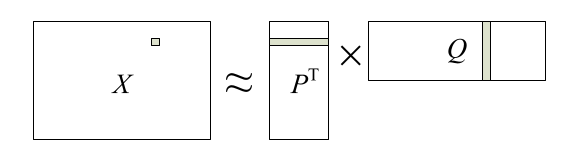
\includegraphics[scale=0.45]{wtmf.png}
            \caption{Разложение TF-IDF матрицы~($X$) на произведение матриц $P$ и $Q$}
            \label{pic:wtmf}
        \end{figure}

        Каждый текст $s_j$ представлен в виде вектора $Q_{\cdot,j}$ размерности $K$, каждое слово $w_i$ представлено в виде вектор $P_{i,\cdot}$.
        Если $X_{ij}=(P_{i,\cdot}, Q_{\cdot,j})$ близко к нулю, то это трактуется как отсутствующее слово.

        Задачей метода является минимизация целевой функции ($\lambda$ - регуляризирующий член, матрица W определяет вес элементов матрицы X):
        \begin{equation}
            \sum_i \sum_j W_{ij} (P_{i,\cdot} \cdot Q_{\cdot,j} - X_{ij})^2 + \lambda ||P||^2_2 + \lambda ||Q||^2_2.
        \end{equation}

        Для получения векторов $P_{i,\cdot}$ и $Q_{\cdot,j}$ используется алгоритм описанный в статье~\cite{matrix_approximation}.
        Сначала P и Q инициализируются случайными числами. Затем запускается итеративный пересчёт P и Q по следующим формулам (эффективный способ расчёта описан в \cite{steck_recommender}):
        \begin{equation}
            P_{i, \cdot} = (Q W'_i Q^T + \lambda I)^{-1} Q W'_i X_{i,\cdot}^T,
        \end{equation}
        \begin{equation}
            Q_{\cdot, j} = (P W'_j P^T + \lambda I)^{-1} P W'_j X_{j,\cdot}.
        \end{equation}
        Здесь $W'_i = diag(W_{i, \cdot})$ - диагональная матрица полученная из $i$-ой строчки матрицы $W$,
        аналогично $W'_j = diag(W_{\cdot, j})$ - диагональная матрица полученная из $j$-ого столбца матрицы $W$.
        Матрица $W$ определяется следующим образом:
        \begin{gather}
            W_{ij} =
            \begin{cases}
                1, ~~if~X_{ij} \neq 0, \nonumber \\
                w_m, ~~otherwise.
            \end{cases},
        \end{gather}
        где $w_m$ положительно и $w_m << 1$.

        Столбцы построенной матрицы Q представляют собой вектора для сравнения текстов между собой.
        Тексту, на основе которого построена $i$-я строка TF-IDF матрицы $X$, в соответствие ставится $i$-й столбей матрицы Q.

        В статье предложен подход для поиска семантической близости текстов, который на небольших текстах работает лучше чем подход, основанный на частотности слов.

    \subsubsection{Метод WTMF-G}
    \label{subsubsec:wtmfg_review}
        %\subsubsection{Метод WTMF-G}
        Метод WTMG-G решает задачу установления связей между твитами и новостными статьями, путём построения модели, которая учитывает неявные связи между текстами,
         предложен в статье~\cite{linking_base}.

        Метод WTMF-G~(WTMF on Graphs) представляет собой доработанный метод WTMF, позволяющий хорошо моделировать семантику коротких текстов,
        но не учитывающий некоторые специфичные для твитов и новостей характеристики, которыми обладает исходная выборка и
        которые взаимосвязаны с семантической близостью текстов:
        \begin{enumerate}
            \item хештеги, которые являются прямым указанием на смысл твита;
            \item именованные сущности, которые с высокой точностью можно извлекать из новостей;
            \item информацию о времени публикации твитов и новостей.
        \end{enumerate}
        Метод WTMF-G расширяет возможности метода WTMF, путём учёта взаимосвязи текстов на основе специфичных для твитов и новостных статей характеристик,
        то есть позволяет учесть информацию о взаимосвязи текст-текст.

        Для решения задачи необходимо иметь эталонный набор данных, на котором будет производится оценка качества полученного решения.
        Сначала за общий период времени собираются твиты и новости.
        Для твита помимо текста хранится информация о времени публикации и авторе работы. Для новости хранится время публикации, заколовок, краткое изложение и URL.
        На основе собранной информации строится набор данных, который состоит из трёх частей:
        \begin{enumerate}
            \item множество новостей~---~все собранные новости;
            \item множество связей твит-новость, под связью подразумевается явное указание URL новости в тексте твита;
            \item множество твитов~--~все твиты, имеющие связь с одной из собранных новостей.
        \end{enumerate}
        К построенному набору данных применяется метод WTMF-G~---~то есть метод WTMF, расширенный путём добавления связей текст-текст.
        Добавление связей текст-текст происходит путём модификации регуляризирующего члена $lambda$. Для каждой пары связанных текстов $j_1$ и $j_2$:
        \begin{equation}
            \lambda = \delta \cdot (\dfrac{Q_{\cdot,j_1}\cdot Q_{\cdot,j_2}}{|Q_{\cdot,j_1}|| Q_{\cdot,j_2}|}-1)^2,
        \end{equation}
        коэффициент $\delta$ задаёт степень влияния связей текст-текст.

        Так как новый регуляризирующий член $\lambda$ зависит от $|Q_{\cdot,j}|$, который меняется во время итерации, вводим упрощение: длина вектора $Q_{\cdot,j}$ не изменяется во время итерации.
        Также необходимо модифицировать итеративный процесс построения матриц $P$ и $Q$ следующим образом:
        \begin{equation}
            P_{i, \cdot} = (Q W'_i Q^T + \lambda I)^{-1} Q W'_i X_{i,\cdot}^T,
        \end{equation}
        \begin{equation}
            Q_{\cdot, j} = (P W'_j P^T + \lambda I + \delta  L_j^2 Q_{\cdot,n(j)} diag(L^2_{n(j)})Q_{\cdot,n(j)}^T)^{-1}   (P W'_j X_{j,\cdot} + \delta  L_j Q_{\cdot,n(j)} L_{n(j)}).
        \end{equation}
        В этих формулах $n(j)$~---~список связанных текстов с текстом $j$. $Q_{\cdot,n(j)}$~---~матрица, состоящая из связанных векторов для $Q_{\cdot, j}$.
        $L_j$ - длина вектора $Q_j$ на начало итерации, $L_n(j)$~---~вектор длин векторов связанных с $j$, то есть $Q_{\cdot,n(j)}$, полученный на начало итерации.

        В статье показано, что добавление информации о взаимосвязи текст-текст позволяет повысить качество установления связей между твитами и новостными статьями.
        Качество метода WTMF-G, полученное с использованием метрики MRR~(метрика описана в главе \ref{subsubsec:MRR}), в сравнении с такими популярными подходами как:
        TF-IDF, LDA, WTMF, показано в таблице~\ref{tabular:wtmfg_comparing}.
        Из таблицы~\ref{tabular:wtmfg_comparing} видно, что алгоритм WTMF-G даёт лучшее качество, чем прочие подходы.
        \begin{table}[ht!]
            %\small
            \caption{Значение метрики MRR для различных методов рекомендаций\bigskip}
            \centering

            \label{tabular:wtmfg_comparing}
            \begin{tabular}{|c|c|c|c|c|c|} \hline
                \bf{Метод} & TF-IDF & LDA & WTMF & WTMF-G \\ \hline
                \bf{Значение MRR} & 0.4602 & 0.1313 & 0.4531 & 0.4791 \\ \hline
            \end{tabular}
        \end{table}